\documentclass[letterpaper,12pt]{article}

\usepackage{tabularx} % extra features for tabular environment
\usepackage{amsmath}  % improve math presentation
\usepackage{graphicx} % takes care of graphic including machinery
\usepackage[margin=1in,letterpaper]{geometry} % decreases margins
\usepackage[final]{hyperref} % adds hyper links inside the generated pdf file
\usepackage{ctex}
\usepackage{titlesec}
%\usepackage{CJKutf8, CJK}
\usepackage{makecell}                 % 三线表-竖线
\usepackage{booktabs}                 % 三线表-短细横线
% \usepackage{natbib}
\usepackage{graphicx}				  % 表格单元格逆时针
\usepackage{multirow}				  % 合并单元格
\usepackage{array}
\usepackage{amssymb}				  % 勾
\usepackage{amsmath}
\usepackage{longtable}                % 导入 longtable 宏包,表格自动换行
\usepackage{caption}
\usepackage{subcaption}               % 设置子图
\usepackage{color}					  % 文本颜色包
\usepackage{xcolor}
\usepackage{bbm}					  % 输入指示函数
\usepackage{tablefootnote}			  % 表格注释
\usepackage{pythonhighlight}

\usepackage{listings}                 % 导入代码块
\usepackage{xcolor}
\lstset{
	numbers=left, 
	tabsize=1,
	columns=flexible, 
	numberstyle=  \small, 
	keywordstyle= \color{ blue!70},
	commentstyle= \color{red!50!green!50!blue!50}, 
	frame=shadowbox, % 阴影效果
	rulesepcolor= \color{ red!20!green!20!blue!20} ,
	escapeinside=``, % 英文分号中可写入中文
	xleftmargin=2em,
	xrightmargin=2em, 
	aboveskip=1em,
} 

\hypersetup{
	colorlinks=true,       % false: boxed links; true: colored links
	linkcolor=blue,        % color of internal links
	citecolor=blue,        % color of links to bibliography
	filecolor=magenta,     % color of file links
	urlcolor=blue         
}
%++++++++++++++++++++++++++++++++++++++++
\titleformat{\section}{\Large\bfseries\songti}{\thesection}{1em}{}
\titleformat{\subsection}{\large\bfseries\songti}{\thesubsection}{1em}{}
\titleformat{\subsubsection}{\normalsize\bfseries\songti}{\thesubsubsection}{1em}{}
\titleformat{\paragraph}{\small\bfseries\songti}{\paragraph}{1em}{}
\titleformat{\subparagraph}{\footnotesize\bfseries\songti}{\subparagraph}{1em}{}

\begin{document}
	
	
	\title{\songti \zihao{4}高级人工智能课程汇报}
	\author{信息科学与工程学院 \\ \textrm{Gu Rui} \\ 220220942871}
	\date{\textrm{June 11 2023}}
	\maketitle
	
	\renewcommand{\figurename}{Figure} % 可以重新定义abstract,因为ctex会覆盖thebibliography
	% 	\begin{abstract}
		%		In this experiment we studied a very important physical effect by measuring the
		%		dependence of a quantity $V$ of the quantity $X$ for two different sample
		%		temperatures.  Our experimental measurements confirmed the quadratic dependence
		%		$V = kX^2$ predicted by Someone's first law. The value of the mystery parameter
		%		$k = 15.4\pm 0.5$~s was extracted from the fit. This value is
		%		not consistent with the theoretically predicted $k_{theory}=17.34$~s. We attribute %this
		%		discrepancy to low efficiency of our $V$-detector.
		%	\end{abstract}
	\renewcommand{\contentsname}{Contents}
	\renewcommand{\tablename}{Table}
	\tableofcontents  % 自动生成目录
	
	\section{第一题:训练RNN模型}
	
		\subsection{结果说明}
	
			一开始的尝试是手动修改超参数,依次把hidden\_size, seq\_lengths, learning\_rate手动修改为4组见Fig. \ref{fig: parameter_tuning},返回文本结果Fig. \ref{fig: RNN_result}
	
			
			\begin{figure}[htbp] 
				% read manual to see what [ht] means and for other possible options
				\centering 
				% \includegraphics[width=0.8\columnwidth]{GLADNet}
				\begin{subfigure}{0.19\textwidth}
					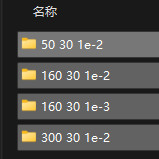
\includegraphics[width=\linewidth]{RNN/parameter_tuning}
					\captionsetup{font=scriptsize}
					\caption{parameter tuning}
					\label{fig: parameter_tuning}
				\end{subfigure} \\
				\begin{subfigure}{0.45\textwidth}
					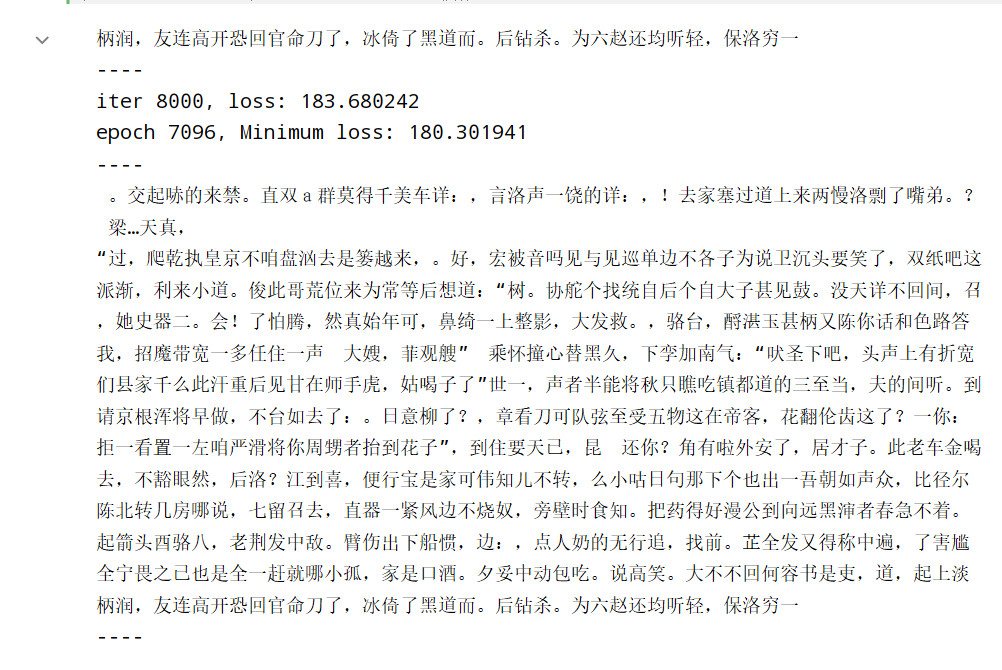
\includegraphics[width=\linewidth]{RNN/result_1}
					\captionsetup{font=scriptsize}
					\caption{50 30 1e-2}
					\label{fig: RNN_result_1}	
				\end{subfigure}
				\begin{subfigure}{0.45\textwidth}
					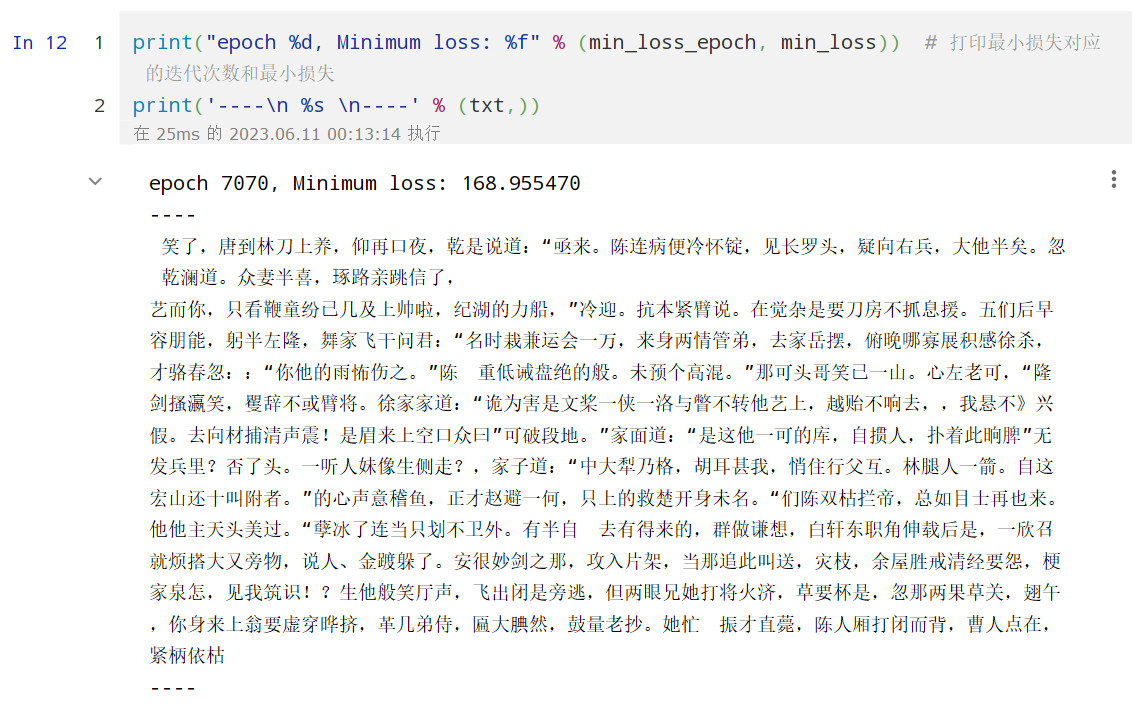
\includegraphics[width=\linewidth]{RNN/result_2}
					\captionsetup{font=scriptsize}
					\caption{160 30 1e-2}
					\label{fig: RNN_result_2}	
				\end{subfigure} \\
				\begin{subfigure}{0.45\textwidth}
					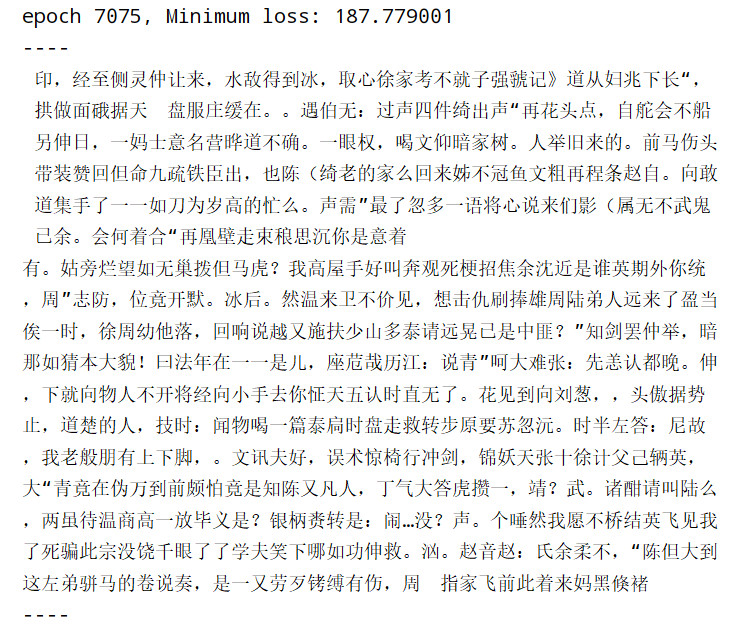
\includegraphics[width=\linewidth]{RNN/result_3}
					\captionsetup{font=scriptsize}
					\caption{160 30 1e-3}
					\label{fig: RNN_result_3}	
				\end{subfigure}
				\begin{subfigure}{0.45\textwidth}
					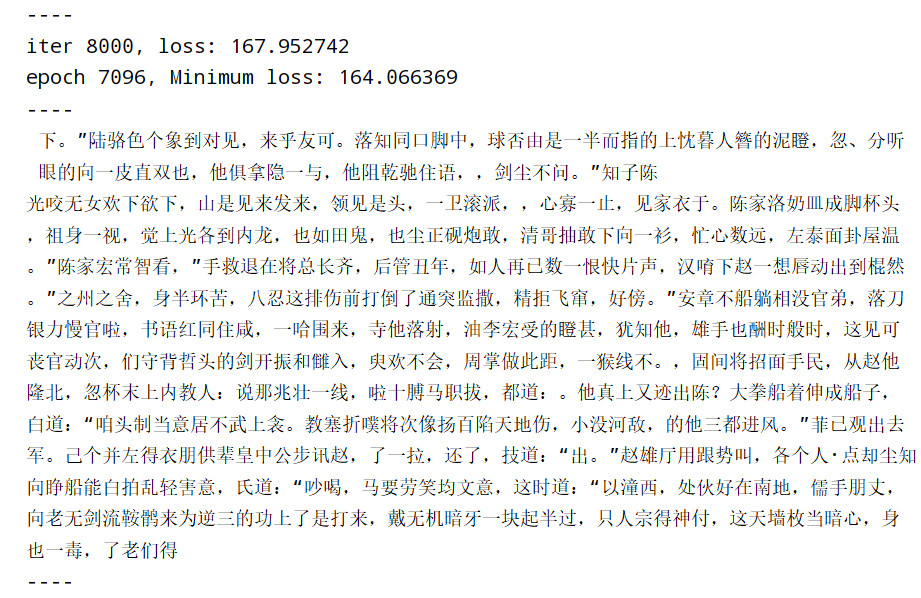
\includegraphics[width=\linewidth]{RNN/result_4}
					\captionsetup{font=scriptsize}
					\caption{300 30 1e-2}
					\label{fig: RNN_result_4}	
				\end{subfigure}
				\captionsetup{font=scriptsize}
				\caption{
					\label{fig: RNN_result} % spaces are big no-no withing labels
						% things like fig: are optional in the label but it helps
						% to orient yourself when you have multiple figures,
						% equations and tables
						RNN下实现的四组调参结果。
				}
			\end{figure}
			
			
			\subsubsection{代码说明}
	
			这里的调参依赖于手动调参,即手动修改超参数。(完整代码见\footnote{https://github.com/npukujui11/AI\_2023/blob/main/RNN.ipynb})
			
			\begin{python}
				# 模型超参数
				hidden_size = 1609 # 隐藏层的神经元数量(50 到 1000 之间)
				seq_length = 30 # RNN的展开步数(25 到 100 之间)
				learning_rate = 1e-3 # 学习率(1e-2 到 1e-5 之间)
			\end{python}
			
			
			训练循环退出条件设定为,损失函数在1000个迭代内,不再减小即退出循环,输出其中最小的损失结果
			\begin{python}
				# 检查损失是否不再减小
				if smooth_loss < min_loss:  # 损失减小
				min_loss = smooth_loss  # 更新最小损失
				min_loss_epoch = n  # 更新最小损失对应的迭代次数
				no_decrease_count = 0  # 重置连续损失不减小的计数器
				else:
				no_decrease_count += 1  # 连续损失不减小的计数器加1
				if no_decrease_count >= 1000:  # 连续损失不减小的计数器达到1000
				break  # 停止训练
			\end{python}
			
			手动调参相对来说比较缓慢,因此重新改写了一下训练调整超参数的代码,首先是把模型超参数设置为一个范围,然后按照设定的步长,采用三个for循环,对超参数进行遍历,这样可以不需要频繁的手动调参。主要代码如下,相较于之前,增加一条退出训练循环的条件,即连续10000个epoch,但是loss的整数位没有减少,即退出训练。这样能明显的加快在调整超参数情况下的训练速度。(详细代码见\footnote{https://github.com/npukujui11/AI\_2023/blob/main/RNN.py})
			\begin{python}
				# 模型超参数(要修改的话,请修改这里 by Gu Rui)
				hidden_sizes = range(50, 1001, 50)  # Hidden layer size
				seq_lengths = range(25, 101, 10)  # RNN sequence length
				learning_rates = [1e-2, 1e-3, 1e-4, 1e-5]  # Learning rate
				
				# 超参数范围
				hidden_sizes = list(range(50, 1001, 50))
				seq_lengths = list(range(25, 101, 10))
				learning_rates = [1e-2, 1e-3, 1e-4, 1e-5]
				
				results = []  # 保存每次训练的结果
				
				for hidden_size in hidden_sizes:
					for seq_length in seq_lengths:
						for learning_rate in learning_rates:
							# 初始化模型参数和训练循环
							# ...
				
							# 训练循环
							prev_loss = None  # 上一个epoch的整数位损失函数值
							no_decrease_count = 0  # 连续整数位没有减少的计数器
				
							while True:
								# ...
					
								# 检查损失是否不再减小
								if smooth_loss < min_loss:  # 损失减小
								min_loss = smooth_loss  # 更新最小损失
								min_loss_epoch = n  # 更新最小损失对应的迭代次数
								no_decrease_count = 0  # 重置连续损失不减小的计数器
								else:
								no_decrease_count += 1  # 连续损失不减小的计数器加1
								if no_decrease_count >= 1000:  # 连续损失不减小的计数器达到20000
								break  # 停止训练
					
								# 判断是否满足终止条件
								if no_decrease_count >= 10000:
								break
					
								# 检查整数位损失函数是否减少
								if prev_loss is not None and int(smooth_loss) >= int(prev_loss):
								no_decrease_count += 1
								else:
								no_decrease_count = 0
					
								prev_loss = smooth_loss
				
							# 保存结果
							result = {
								'hidden_size': hidden_size,
								'seq_length': seq_length,
								'learning_rate': learning_rate,
								'min_loss': min_loss,
								'min_loss_epoch': min_loss_epoch
							}
							results.append(result)
			\end{python}
			
			但是依然存在问题,就是发现hidden\_size的步长还是设置小了,这样下来一组代码运行下来,实际上相当于调整$19 \times 7 \times 4 = 532$次超参数,因为是采用CPU运行,所以一次下来运行时间要一整天(运行环境为12th Gen Intel(R) i7-12700F),解决方法是把hidden\_size或seq\_length调大,或者再增加额外的训练循环退出条件,如限定epoch的值(实际上会发现,当迭代次数很大时,loss的值只会在小数点后两位数下减少收敛,如Fig. \ref{fig: RNN_quit}。同时,能明显的观察到在,迭代次数多,往往性能不是最好,如Fig. \ref{fig: quit_2}和Fig. \ref{fig: quit_3}所示,二者的迭代次数都很大,但是loss值却仍然接近。此外,能从Fig. \ref{fig: RNN_quit}中明显看到,迭代次数大,往往生成文本的效果都比较差,基本上乱码居多,说明此时模型参数设置不佳,从寻找最优超参数的角度出发,应该抛弃训练,进入下一个超参数训练循环)。
			
			\begin{figure}[htbp] 
				% read manual to see what [ht] means and for other possible options
				\centering 
				% \includegraphics[width=0.8\columnwidth]{GLADNet}
				\begin{subfigure}{0.23\textwidth}
					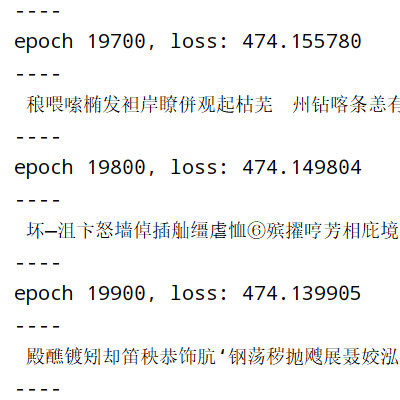
\includegraphics[width=\linewidth]{RNN/quit_1}
					\captionsetup{font=scriptsize}
					\caption{scenario one }
					\label{fig: quit_1}
				\end{subfigure}
				\begin{subfigure}{0.23\textwidth}
					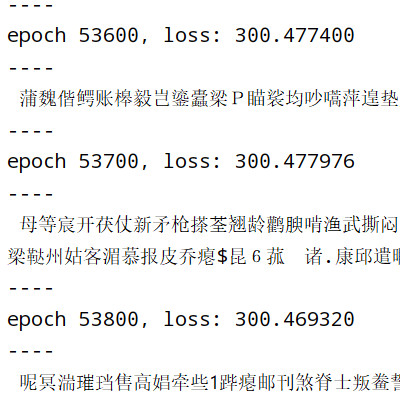
\includegraphics[width=\linewidth]{RNN/quit_2}
					\captionsetup{font=scriptsize}
					\caption{scenario two}
					\label{fig: quit_2}	
				\end{subfigure}
				\begin{subfigure}{0.23\textwidth}
					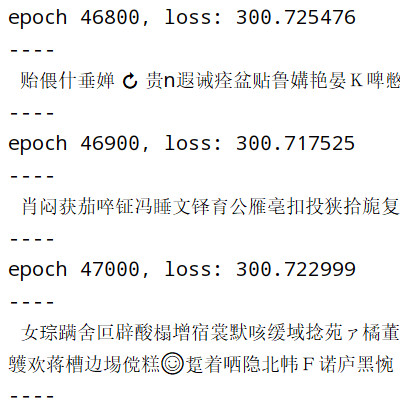
\includegraphics[width=\linewidth]{RNN/quit_3}
					\captionsetup{font=scriptsize}
					\caption{scenario three}
					\label{fig: quit_3}	
				\end{subfigure}
				\begin{subfigure}{0.23\textwidth}
					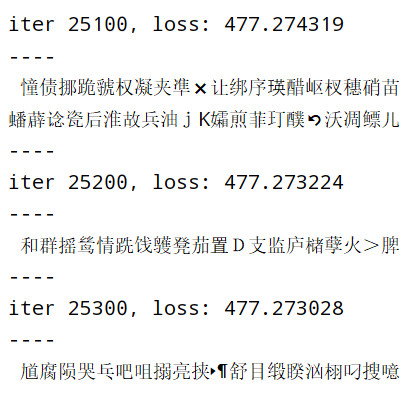
\includegraphics[width=\linewidth]{RNN/quit_4}
					\captionsetup{font=scriptsize}
					\caption{scenario four}
					\label{fig: quit_4}	
				\end{subfigure}
				\captionsetup{font=scriptsize}
				\caption{
					\label{fig: RNN_quit} % spaces are big no-no withing labels
					% things like fig: are optional in the label but it helps
					% to orient yourself when you have multiple figures,
					% equations and tables
					RNN下四组训练过程截图。
				}
			\end{figure}
	
		\subsection{模型设计}
		
		这里遵循题目规则,只调用了numpy,未调用第三方RNN库。同时参考示例代码(见下列代码),实现了一个含有两层隐藏层的通用RNN模型,手动修改实现了模型参数的初始化、前向传播、反向传播和参数更新(代码\footnote{https://github.com/npukujui11/AI\_2023/blob/main/RNN.py}中的Loss Function和Result Sampling部分)。
		
		\begin{python}
			import numpy as np
			
			# 模型超参数
			hidden_size = 100  # 隐藏层神经元的数量
			seq_length = 25  # RNN展开的步数
			learning_rate = 1e-1  # 学习率
			
			# 初始化模型参数
			Wxh = np.random.randn(hidden_size, vocab_size) * 0.01  # 输入到隐藏层的权重
			Whh = np.random.randn(hidden_size, hidden_size) * 0.01  # 隐藏层到隐藏层的权重
			Why = np.random.randn(vocab_size, hidden_size) * 0.01  # 隐藏层到输出层的权重
			bh = np.zeros((hidden_size, 1))  # 隐藏层的偏置
			by = np.zeros((vocab_size, 1))  # 输出层的偏置
			
			# 训练循环
			for i in range(num_iterations):
				# 在每个训练迭代中,根据输入序列和目标序列计算梯度
				# ...
				
				# 参数更新
				# ...
				
				# 模型采样
				if i % sample_interval == 0:
				# 使用当前模型参数进行采样
				# ...
			
			# 定义模型采样函数
			def sample(hprev, seed_ix, n):
				# ...
				return sampled_sequence
			
		\end{python}
	
			
	
	\section{问题二:实现WRNN模型}
	
	观察题目给出的模型图,我不难看出,这是一个包含两层隐藏层$a$、$b$(其中,a和b为LSTM)的RNN网络,其中$f_1,f_2$我选用sigmoid函数,$f_3$我选用softmax函数。
	
	\begin{figure}[htbp] 
		% read manual to see what [ht] means and for other possible options
		\centering 
		% \includegraphics[width=0.8\columnwidth]{GLADNet}
		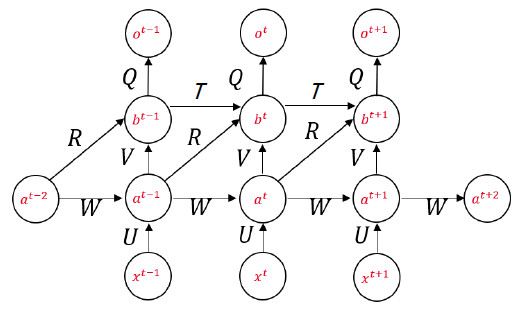
\includegraphics[width=0.5\linewidth]{network}
		\captionsetup{font=scriptsize}
		\label{network}
		\captionsetup{font=scriptsize}
		\caption{
			\label{fig: WRNN_network} % spaces are big no-no withing labels
			% things like fig: are optional in the label but it helps
			% to orient yourself when you have multiple figures,
			% equations and tables
			WRNN网络结构图。
		}
	\end{figure}
	
	Eq.\ref{eq: Forward propagation formula_1}给出了从输入层$x$到第一层隐藏层$a$的前向传播过程。Eq.\ref{eq: Forward propagation formula_2}给出了从隐藏层$a$到第二层隐藏层$b$的前向传播过程。Eq.\ref{eq: Forward propagation formula_3}给出了从隐藏层$b$到输出层$o$的前向传播过程。
	
	\begin{equation}
		\begin{aligned}
			a^t = f_1(Ux^t+Wa^{t-1}+s_1)
		\end{aligned}
		\label{eq: Forward propagation formula_1}
	\end{equation}
	
	\begin{equation}
		\begin{aligned}
			b^t = f_2(Va^t+Ra^{t-1}+Tb^{t-1}+s_2)
		\end{aligned}
		\label{eq: Forward propagation formula_2}
	\end{equation}
	
	\begin{equation}
		\begin{aligned}
			o^t = f_3(Qb^t+s_2)
		\end{aligned}
		\label{eq: Forward propagation formula_3}
	\end{equation}
	
	前向传播过程的主要代码如下
	
	\begin{python}
		# 前向传播过程
		for t in range(len(inputs)):  # 对序列中的每个字符
			x = np.zeros((vocab_size, 1))  # 初始化输入
			x[inputs[t]] = 1  # 将当前字符对应的输入置为1
			a[t] = sigmoid(np.dot(Ux, x) + np.dot(Wx, a[t - 1]) + s1)  # 计算隐藏层a
			b[t] = sigmoid(np.dot(Vx, a[t]) + np.dot(Rx, a[t - 1]) + np.dot(Tx, b[t - 1]) + s2)  # 计算隐藏层b
			o[t] = softmax(np.dot(Qx, b[t]) + s3)  # 计算输出层
			loss += -np.log(o[t][targets[t], 0])  # softmax (cross-entropy loss) 计算损失
	\end{python}
	
	由Eq.\ref{eq: Forward propagation formula_1}, Eq.\ref{eq: Forward propagation formula_2}, Eq.\ref{eq: Forward propagation formula_3}不难得出整个反向传播的过程,对于每一个时间步$t$(从后往前),
	
	$do = o^{(t)}$
	
	$do[targets[t]] = do[targets[t]] - 1$(误差传播到输出层)
	
	$dQx = dQx + do \cdot b^{(t)T}$(误差传播到LSTM隐藏层与输出层的权重矩阵)
	
	$ds_3 = ds_3 + do$(误差传播到输出层的偏置项)
	
	$dbt = Qx^T \cdot do$(误差传播到LSTM隐藏层)
	
	$dbt_{\text{raw}} = dbt \cdot (1 - b^{(t)} \cdot b^{(t)})$(通过tanh非线性函数的误差反向传播)
	
	$dVx = dVx + dbt_{\text{raw}} \cdot a^{(t)T}$(误差传播到LSTM隐藏层与RNN隐藏层的权重矩阵)
	
	$dRx = dRx + dbt_{\text{raw}} \cdot a^{(t-1)T}$(误差传播到RNN隐藏层与LSTM隐藏层的权重矩阵)
	
	$dTx = dTx + dbt_{\text{raw}} \cdot b^{(t-1)T}$(误差传播到LSTM隐藏层自连接的权重矩阵)
	
	$ds_2 = ds_2 + dbt_{\text{raw}}$(误差传播到LSTM隐藏层的偏置项)
	
	$dat = Vx^T \cdot dbt_{\text{raw}} + Rx^T \cdot dbt_{\text{raw}}$(误差传播到RNN隐藏层)
	
	$dUx = dUx + dat_{\text{raw}} \cdot x^T$(误差传播到输入权重矩阵)
	
	$ds_1 = ds_1 + dat_{\text{raw}}$(误差传播到RNN隐藏层的偏置项)
	
	
	因此,反向传播过程的主要代码如下
	
	\begin{python}
		# 后向传播过程
		dUx, dWx, dVx, dRx, dTx, dQx = np.zeros_like(Ux), np.zeros_like(Wx), np.zeros_like(Vx), \
		np.zeros_like(Rx), np.zeros_like(Tx), np.zeros_like(Qx)  # 初始化参数梯度
		
		ds1, ds2, ds3 = np.zeros_like(s1), np.zeros_like(s2), np.zeros_like(s3)  # 初始化偏置梯度
		
		for t in reversed(range(len(inputs))):  # 对序列中的每个字符
			do = o[t].copy()
			do[targets[t]] -= 1  # backprop into o
			
			dQx += np.dot(do, b[t].T)  # backprop into Qx
			ds3 += do  # backprop into s3
			
			dbt = np.dot(Qx.T, do)  # backprop into b
			dbt_raw = dbt * (1 - b[t] * b[t])  # backprop through tanh nonlinearity
			
			dVx += np.dot(dbt_raw, a[t].T)  # backprop into Vx
			dRx += np.dot(dbt_raw, a[t - 1].T)  # backprop into Rx
			dTx += np.dot(dbt_raw, b[t - 1].T)  # backprop into Tx
			ds2 += dbt_raw  # backprop into s2
			
			dat = np.dot(Vx.T, dbt_raw) + np.dot(Rx.T, dbt_raw)  # backprop into a
			dat_raw = dat * (1 - a[t] * a[t])  # backprop through tanh nonlinearity
			
			dUx += np.dot(dat_raw, x.T)  # backprop into Ux
			dWx += np.dot(dat_raw, a[t - 1].T)  # backprop into Wx
			ds1 += dat_raw  # backprop into s1
	\end{python}
	
	此外为了防止梯度爆炸,需要加入下列代码,以防止潜在的梯度溢出的情况。
	
	\begin{python}
		for dparam in [dUx, dWx, dVx, dRx, dTx, dQx, ds1, ds2, ds3]:  # clip to mitigate exploding gradients
			np.clip(dparam, -5, 5, out=dparam)  # clip to mitigate exploding gradients
	\end{python}
	
	
	\section{问题三:实现WRNN模型}
	
	WRNN代码\footnote{https://github.com/npukujui11/AI\_2023/blob/main/WRNN.py}实现,在这部分的工作,我主要是重写了lossFun和sample函数,次要工作是修改超参数训练策略和增加训练循环的退出条件。
	
	其中在lossFun函数中我实现了WRNN参数的初始化、前向传播、损失计算、反向传播。
	
	Fig. \ref{fig: WRNN_result}给出了5组对比实验结果。
	
	\begin{figure}[htbp] 
		% read manual to see what [ht] means and for other possible options
		\centering 
		% \includegraphics[width=0.8\columnwidth]{GLADNet}
		\begin{subfigure}{0.3\textwidth}
			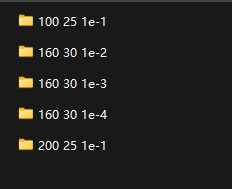
\includegraphics[width=\linewidth]{WRNN/parameter_tuning}
			\captionsetup{font=scriptsize}
			\caption{parameter\_tuning}
			\label{fig: WRNN_parameter_tuning}
		\end{subfigure} 
		\begin{subfigure}{0.3\textwidth}
			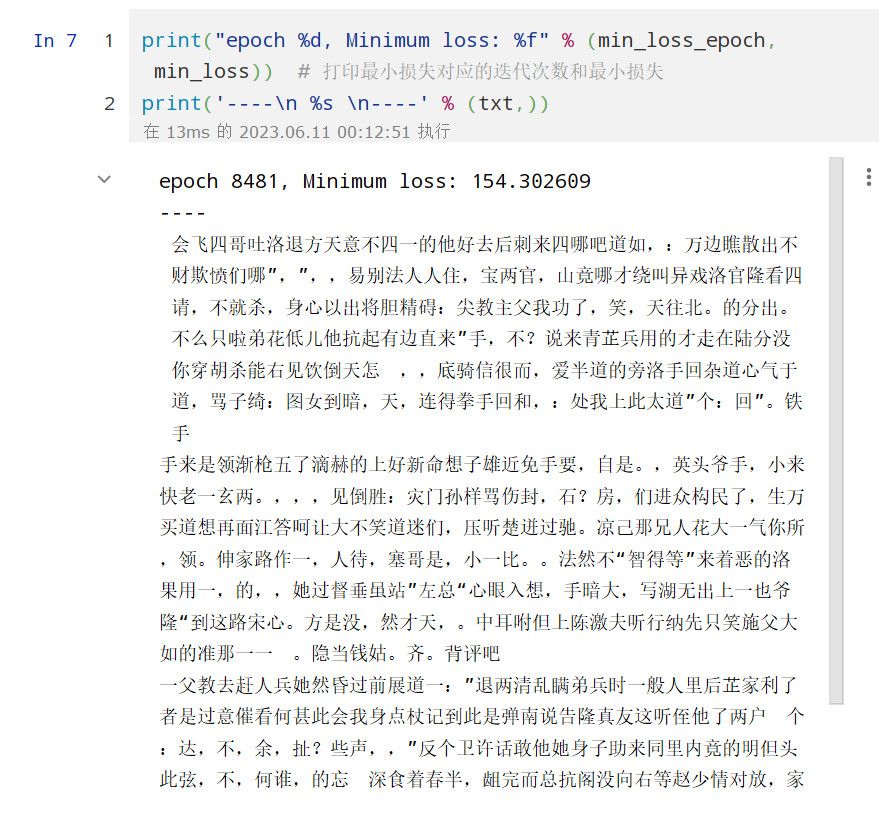
\includegraphics[width=\linewidth]{WRNN/result_1}
			\captionsetup{font=scriptsize}
			\caption{100 25 1e-1}
			\label{fig: WRNN_result_1}	
		\end{subfigure} 
		\begin{subfigure}{0.3\textwidth}
			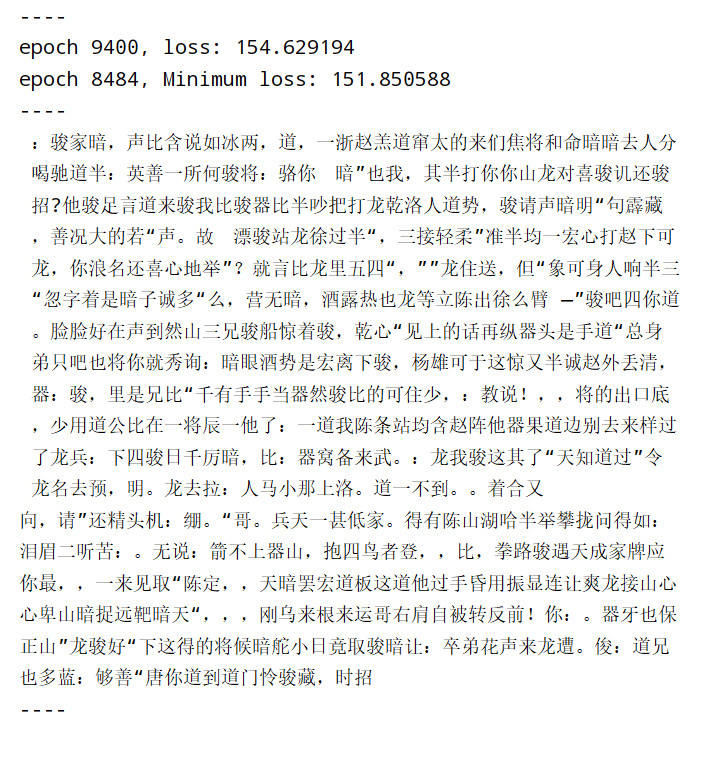
\includegraphics[width=\linewidth]{WRNN/result_5}
			\captionsetup{font=scriptsize}
			\caption{200 25 1e-1}
			\label{fig: WRNN_result_5}	
		\end{subfigure} \\
		\begin{subfigure}{\textwidth}
			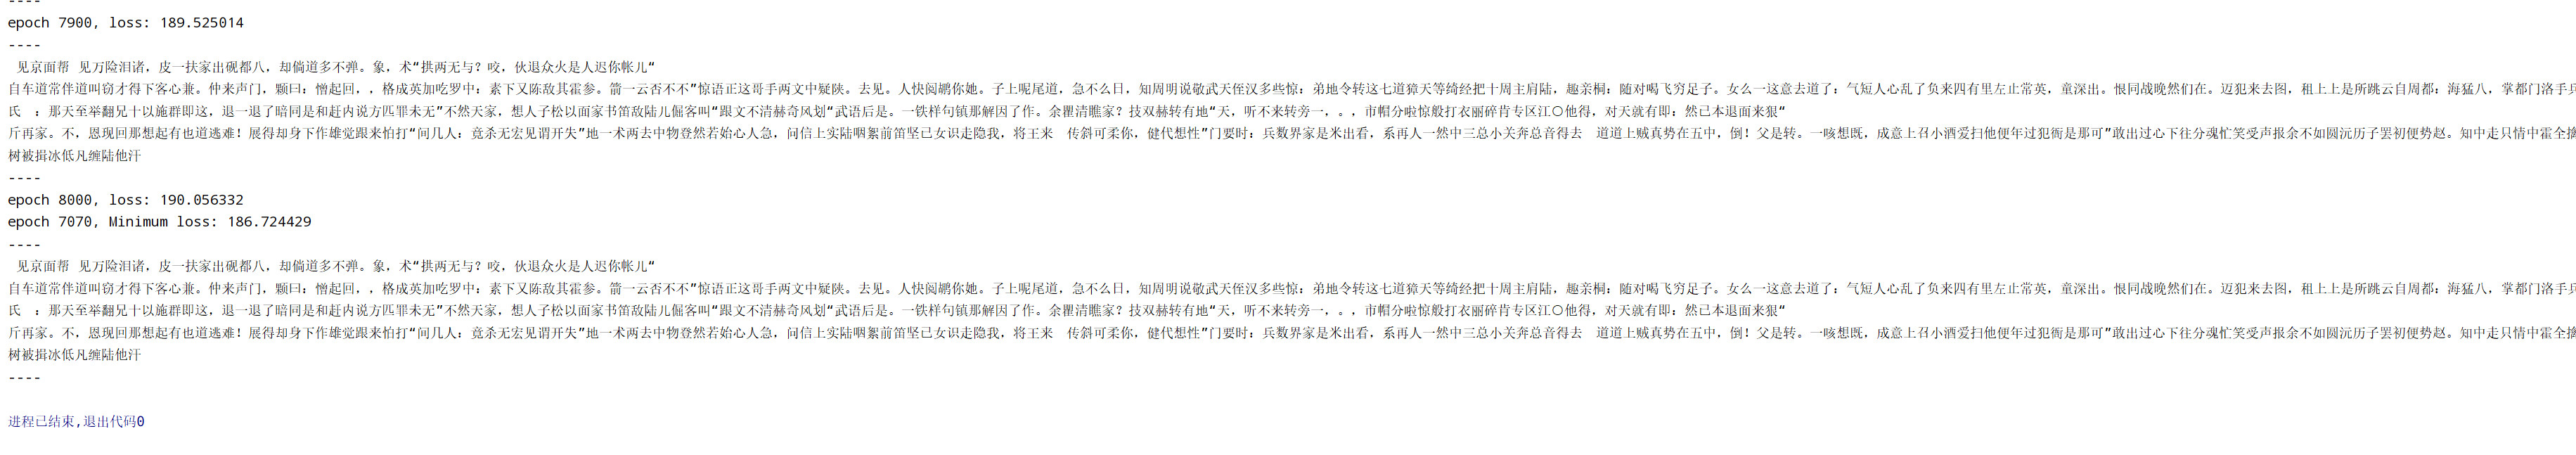
\includegraphics[width=\linewidth]{WRNN/result_2}
			\captionsetup{font=scriptsize}
			\caption{160 30 1e-2}
			\label{fig: WRNN_result_2}	
		\end{subfigure} \\ 
		\begin{subfigure}{\textwidth}
			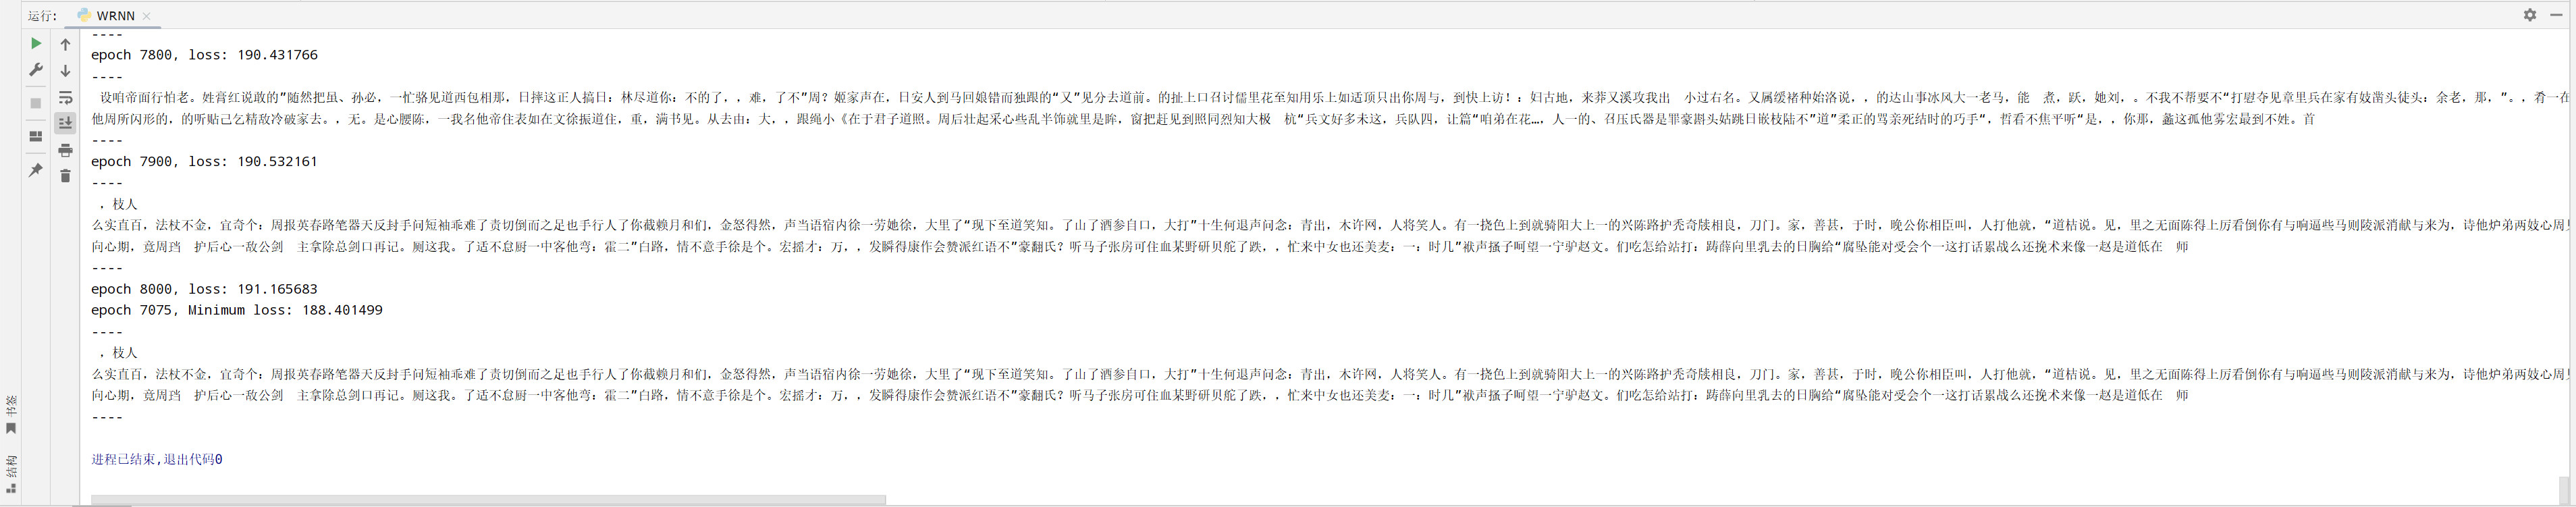
\includegraphics[width=\linewidth]{WRNN/result_3}
			\captionsetup{font=scriptsize}
			\caption{160 30 1e-3}
			\label{fig: WRNN_result_3}	
		\end{subfigure} \\
		\begin{subfigure}{\textwidth}
			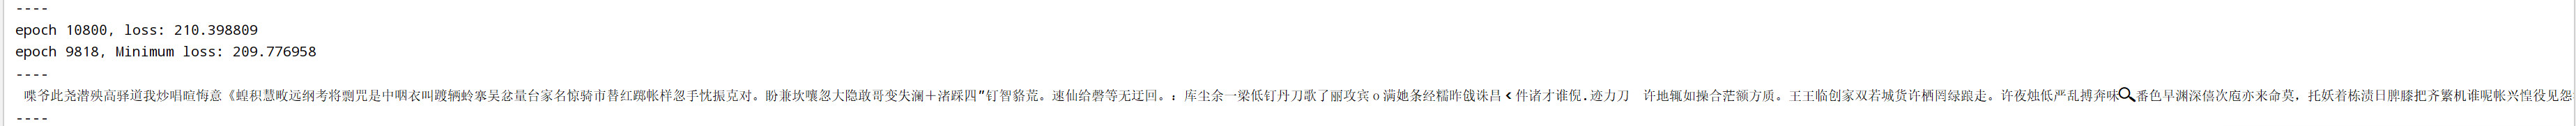
\includegraphics[width=\linewidth]{WRNN/result_4}
			\captionsetup{font=scriptsize}
			\caption{160 30 1e-4}
			\label{fig: WRNN_result_4}	
		\end{subfigure}
		\captionsetup{font=scriptsize}
		\caption{
			\label{fig: WRNN_result} % spaces are big no-no withing labels
			% things like fig: are optional in the label but it helps
			% to orient yourself when you have multiple figures,
			% equations and tables
			WRNN下实现的四组调参结果。因为后期修改了调参策略(在第一题中提到),所以相对比较全面的对比结果还没有(限于作业提交时间关系,后续可以把结果补上,这里图片中的结果只做一个展示和说明。跑一次,找到一个最优的参数需要3h左右)
		}
	\end{figure}
	
	Fig. \ref{fig: WRNN_result_2}和Fig. \ref{fig: WRNN_result_3}在RNN中有对比实验,loss的值都比RNN的低,或许能够说明在hidden\_layer不是很深的情况下,RNN的效果可能要更好,在不考虑学习率的情况下,从Fig. \ref{fig: WRNN_result_4}和Fig. \ref{fig: WRNN_result_5}的结果中可以推断,随着hidden\_layer的增加,WRNN的效果应该是要优于RNN,但是降低学习率对于RNN和WRNN来说会导致文本出现乱码的情况增多,或者只生成乱码。

	\section{一些说明}
	
	完整的项目在已经上传到GitHub\footnote{https://github.com/npukujui11/AI\_2023}中,上面有个人的提交记录和代码的详细修改记录\footnote{https://github.com/npukujui11/AI\_2023/commits/main}。上面提到的图片都是用Jupyter Notebook跑,但是因为题目限定了无法使用第三方RNN库,所以未使用torch,因而无法使用GPU训练模型。而使用CPU训练的速度,加上手动调参,过于缓慢了,所以对比实验没做完全。考虑到,时间的因素,所以完整的训练过程我并没有使用Jupyter Notebook,RNN.py和WRNN.py一直还在在训练(见Fig. \ref{fig: train})后续完整的结果可以通过邮箱发给老师。
	
	\begin{figure}[htbp] 
		% read manual to see what [ht] means and for other possible options
		\centering 
		% \includegraphics[width=0.8\columnwidth]{GLADNet}
		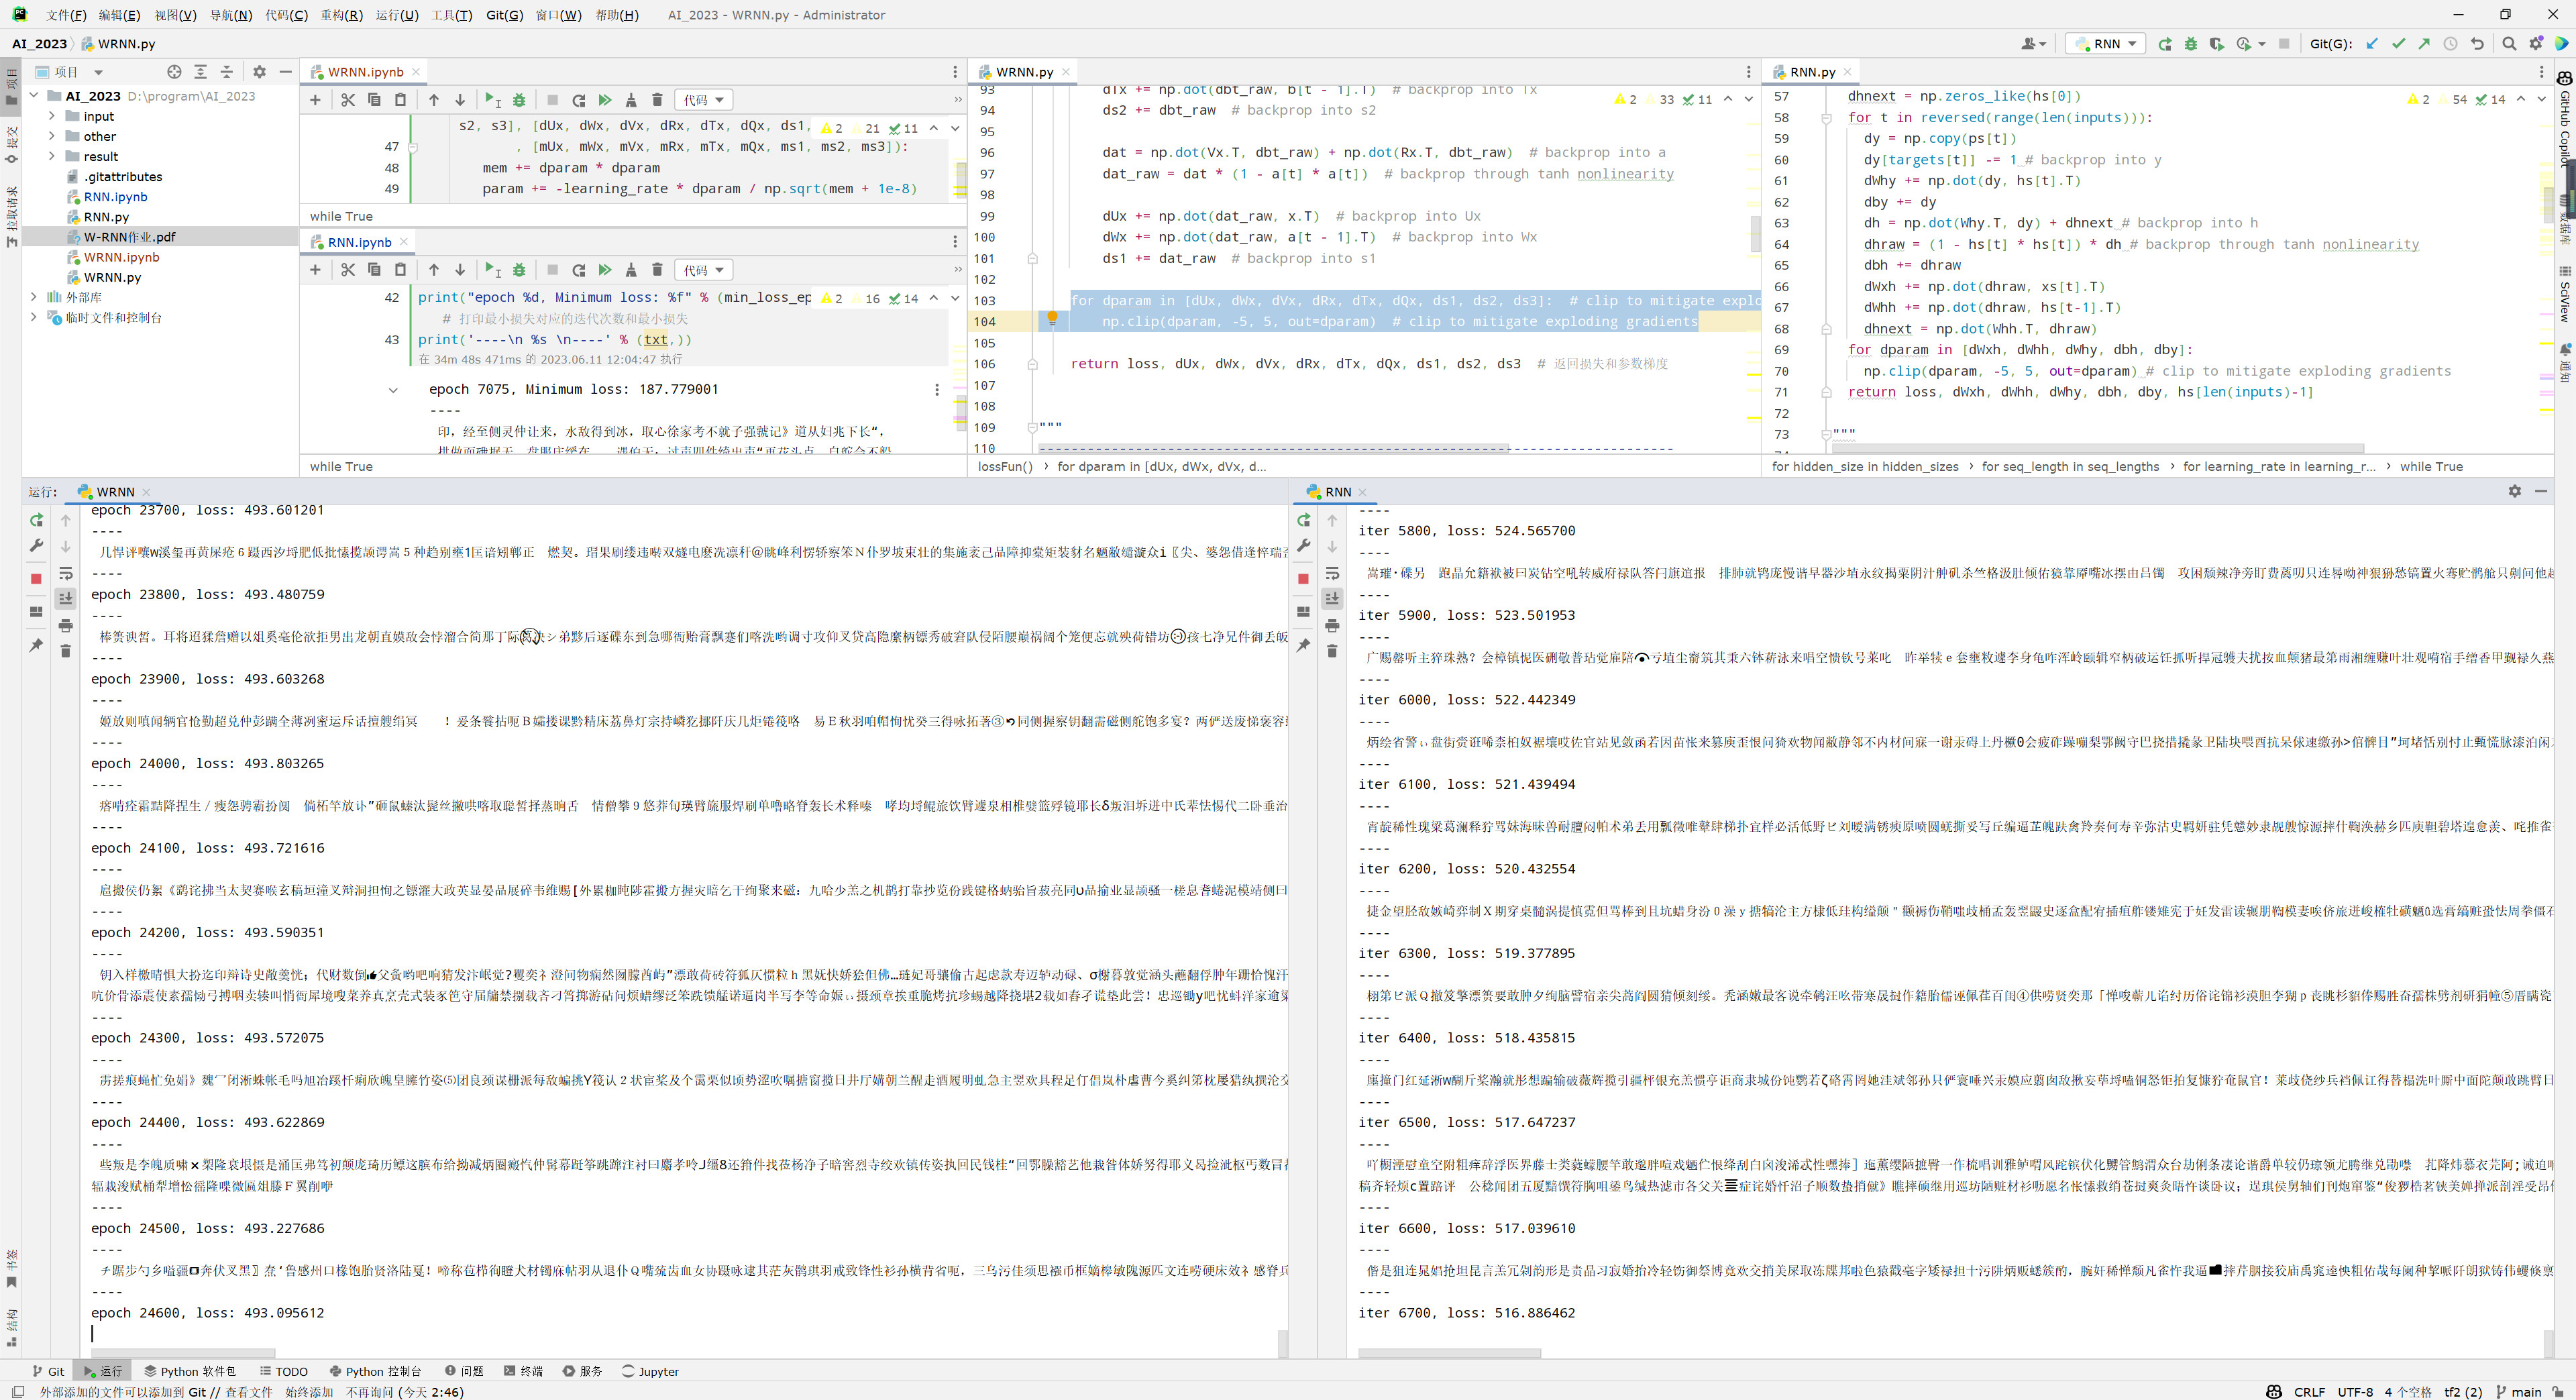
\includegraphics[width=\linewidth]{train}
		\captionsetup{font=scriptsize}
		\label{train}
		\captionsetup{font=scriptsize}
		\caption{
			\label{fig: train} % spaces are big no-no withing labels
			% things like fig: are optional in the label but it helps
			% to orient yourself when you have multiple figures,
			% equations and tables
			运行RNN.py和WRNN.py的PyCharm界面。
		}
	\end{figure}
	
	
	%	\section{Analysis}
	
	%	In this section you will need to show your experimental results. Use tables and
	%	graphs when it is possible. Table~\ref{tbl:bins} is an example.
	
	%	\begin{table}[ht]
		%		\begin{center}
			%			\caption{Every table needs a caption.}
			%			\label{tbl:bins} % spaces are big no-no withing labels
			%			\begin{tabular}{|ccc|} 
				%				\hline
				%				\multicolumn{1}{|c}{$x$ (m)} & \multicolumn{1}{c|}{$V$ (V)} & \multicolumn{1}{c|}{$V$ (V)} \\
				%				\hline
				%				0.0044151 &   0.0030871 &   0.0030871\\
				%				0.0021633 &   0.0021343 &   0.0030871\\
				%				0.0003600 &   0.0018642 &   0.0030871\\
				%				0.0023831 &   0.0013287 &   0.0030871\\
				%				\hline
				%			\end{tabular}
			%		\end{center}
		%	\end{table}
	%	
	%	Analysis of equation~\ref{eq:aperp} shows ...
	%	
	%	Note: this section can be integrated with the previous one as long as you
	%	address the issue. Here explain how you determine uncertainties for different
	%	measured values. Suppose that in the experiment you make a series of
	%	measurements of a resistance of the wire $R$ for different applied voltages
	%	$V$, then you calculate the temperature from the resistance using a known
	%	equation and make a plot  temperature vs. voltage squared. Again suppose that
	%	this dependence is expected to be linear~\cite{Cyr}, and the proportionality coefficient
	%	is extracted from the graph. Then what you need to explain is that for the
	%	resistance and the voltage the uncertainties are instrumental (since each
	%	measurements in done only once), and they are $\dots$. Then give an equation
	%	for calculating the uncertainty of the temperature from the resistance
	%	uncertainty. Finally explain how the uncertainty of the slop of the graph was
	%	found (computer fitting, graphical method, \emph{etc}.)
	%	
	%	If in the process of data analysis you found any noticeable systematic
	%	error(s), you have to explain them in this section of the report.
	%	
	%	It is also recommended to plot the data graphically to efficiently illustrate
	%	any points of discussion. For example, it is easy to conclude that the
	%	experiment and theory match each other rather well if you look at
	%	Fig.~\ref{fig:samplesetup} and Fig.~\ref{fig:exp_plots}.
	%	
	%	\begin{figure}[ht] 
		%		\centering
		%		\includegraphics[width=0.5\columnwidth]{sr_squeezing_vs_detuning}
		%		
		%		% some figures do not need to be too wide
		%		\caption{
			%			\label{fig:exp_plots}  
			%			Every plot must have axes labeled.
			%		}
		%	\end{figure}
	
	
	%	\section{Conclusions}
	%	Here you briefly summarize your findings.
	
	%++++++++++++++++++++++++++++++++++++++++
	% References section will be created automatically 
	% with inclusion of "thebibliography" environment
	% as it shown below. See text starting with line
	% \begin{thebibliography}{99}
		% Note: with this approach it is YOUR responsibility to put them in order
		% of appearance.
		
%		\renewcommand{\refname}{References}
%		
%		
%		%	\begin{thebibliography}{00}
%			
%			%		\bibitem{b1}\label{cite:b1}
%			%		W. Wang, C. Wei, W. Yang and J. Liu, "GLADNet: Low-Light Enhancement Network with Global Awareness," 2018 13th IEEE International Conference on Automatic Face \& Gesture Recognition (FG 2018), Xi'an, China, 2018, pp. 751-755, DOI: 10.1109/FG.2018.00118.
%			
%			%		\bibitem{b2}\label{cite:b2}
%			%		A.\ Mahajan, K.\ Somaraj and M. Sameer, "Adopting Artificial Intelligence Powered ConvNet To Detect Epileptic Seizures," 2020 IEEE-EMBS Conference on Biomedical Engineering and Sciences (IECBES), Langkawi Island, Malaysia, 2021, pp. 427-432, DOI: 10.1109/IECBES48179.2021.9398832.
%			
%			%		\bibitem{Cyr}
%			%		N.\ Cyr, M.\ T$\hat{e}$tu, and M.\ Breton,
%			% "All-optical microwave frequency standard: a proposal,"
%			%		IEEE Trans.\ Instrum.\ Meas.\ \textbf{42}, 640 (1993).
%			
%			
%			
%			%	\end{thebibliography}
%		
%		\bibliographystyle{unsrt}
%		\bibliography{reference}
		
		
	\end{document}
